% !TeX program = pdflatex
% !TeX TS-program = pdflatex
% !TeX TXS-program:compile = txs:///pdflatex/

% !BIB program = biber
% !BIB TS-program = biber
% !TeX TXS-program:bibliography = txs:///biber




%%%%%%%%%%%%%%%%%%%%%%%%%%%%%%%%%%%%%%%%%
%%  FUNDAMENTAL SETTINGS AND PACKAGES  %%
%%%%%%%%%%%%%%%%%%%%%%%%%%%%%%%%%%%%%%%%%


\documentclass[11pt, a4paper, titleabove]{simplecv}

\newcommand{\myname}{Dr. Holger Gerhardt}

\usepackage{xpatch}
\usepackage{ifxetex}  % Detect if engine is XeTeX/XeLaTeX
\usepackage[utf8]{inputenc}  % so that umlauts can be input without having to use TeX code
\usepackage[ngerman, USenglish]{babel}
\usepackage{ragged2e}

\usepackage{calc}
\usepackage{tikz}
\usepackage{tcolorbox}
\usetikzlibrary{positioning}
\usepackage{xcolor}
\definecolor{UBonnBlue}   {RGB}{  7,  82, 154}
\definecolor{UBonnYellow} {RGB}{234, 185,  12}
\definecolor{UBonnGray}   {RGB}{144, 144, 133}
\definecolor{darkgray}    {RGB}{102, 102, 102}
\definecolor{darkred}     {RGB}{153,   0,   0}
\definecolor{neutralgreen}{RGB}{ 28, 166,   0}

\colorlet{SpotColor}{UBonnBlue}

\usepackage{authoraftertitle}

\usepackage[hyphens]{url}
\usepackage[unicode=true]{hyperref}
\hypersetup{
	colorlinks=true,
	linkcolor=black,
	anchorcolor=black,
	citecolor=black,
	filecolor=black,
	menucolor=black,
	runcolor=black,
	urlcolor=SpotColor,
	bookmarks=true,
	bookmarksnumbered=false,
	bookmarksopenlevel=1,
	pdfstartview=Fit,
	pdfpagelayout=SinglePage,
	plainpages=false,
	pdfpagelabels=true,
	pdfauthor=\myname,
	pdftitle={\myname's Curriculum Vitae}
}
\urlstyle{same}
\Urlmuskip = 0mu\relax  % Prevent additional whitespace before/after breakable characters in URLs
\newcommand{\email}[1]{\href{mailto:#1}{\nolinkurl{#1}}}
\newcommand{\doi}[1]{\href{https://doi.org/#1}{#1}}




%%%%%%%%%%%%%%%%%%%
%%  PAGE LAYOUT  %%
%%%%%%%%%%%%%%%%%%%

\raggedbottom

\usepackage{geometry}
\geometry{
	a4paper,
	left=5mm,
	right=30mm,
	top=30mm,
	bottom=30mm
}
\renewcommand{\topicmargin}{57.5mm}
% Make the label right-aligned:
\makeatletter
\renewcommand{\@topic@makelabel}[1]{\hfill\cv@tlab@fnt #1\quad}
\renewcommand{\cv@do@title}{%
	\par\bigskip
	{\noindent\hspace{\topicmargin}\cv@tit@fnt\cv@tit}%
}
\makeatother

% Slightly increase the line spacing
\renewcommand{\baselinestretch}{1.03}

% Footer ==>
\usepackage{pageslts}
\pagenumbering{arabic}
\usepackage{fancyhdr}
\AtBeginDocument{%
	\title{\MyAuthor}%
}
\renewcommand{\headrulewidth}{0pt}
\pagestyle{fancy}
\fancyhf{}
\lfoot{%
	\small\sffamily\color{SpotColor}%
	\makebox[\topicmargin][r]{Page~\thepage\ of~\pageref*{LastPage}\enspace\quad}%
	\textbf{\MyTitle}\enspace\quad%
	\MyDate%
}
% <==

\newenvironment{preventpagebreak}
	{\par\begin{minipage}[t]{\dimexpr\textwidth - \topicmargin\relax}}
	{\end{minipage}\par\vspace{\parskip}}

% Allow for multiline topic labels:
\newcommand{\multiline}[1]{%
	\parbox[t][10pt][t]{\topicmargin-50pt}{\RaggedLeft%
		#1%
		\normalsize\par%
			% So that \baselineskip is of the normal size, see https://tex.stackexchange.com/a/408544
	}%
}




%%%%%%%%%%%%%%%%%%%%%
%%  FONT SETTINGS  %%
%%%%%%%%%%%%%%%%%%%%%


\ifxetex
	\usepackage[protrusion=true, expansion=false]{microtype}
\else
	\usepackage[protrusion=true, expansion=false, kerning=true]{microtype}
	\DisableLigatures[f]{family = {rm*}}
	% Disable the f* ligatures for Charter because the font does not provide sufficient support.
	\DisableLigatures[f]{family = {tt*}}
	% Disable the f* ligatures for Fira Mono because they make no sense for a monospaced font.
	\SetExtraKerning[unit=space]
	{encoding=*, family=*, series=*, size={*, normalsize, footnotesize}, font = */*/*/*/*}
	{\textemdash = {325, 325},
		/ = {100, 100},
		: = { 50,   0},
		; = { 50,   0}}
\fi

% Enabling slightly reduced font for CAPS:
\usepackage{relsize}
\renewcommand\RSpercentTolerance{1}
\ifxetex
	\newcommand{\caps}[1]{\textscale{0.96}{\addfontfeature{LetterSpace=5}\MakeUppercase{#1}}}
\else
	\newcommand{\caps}[1]{\textscale{0.96}{\textls[35]{\MakeUppercase{#1}}}}
\fi

\titlefont{\Large\sffamily\bfseries\color{SpotColor}}
\newcommand{\mysectionfont}{\large\sffamily\bfseries}
\sectionfont{\mysectionfont\color{SpotColor}}
\topictitlefont{\rmfamily}

\newcommand{\commabbrev}[1]{\textsf{#1}}

\ifxetex
	\usepackage{fontspec}
	\usepackage[proportional, oldstyle, scale=0.94]{sourceserifpro}
	\newcommand{\sansseriffont}{WorkSans}
		% Open-source font, available at https://github.com/weiweihuanghuang/Work-Sans
	\setsansfont{\sansseriffont-Regular}[
		ItalicFont = {\sansseriffont-Italic},
		BoldFont ={\sansseriffont-SemiBold},
		BoldItalicFont = {\sansseriffont-SemiBoldItalic},
		Numbers = {Proportional, OldStyle},
		Scale = 0.90,
		LetterSpace = -2
	]
	\topiclabelfont{%
		\small\sffamily% \bfseries\color{SpotColor}%
	}
\else
	%\usepackage[scale=0.88]{plex-sans}
	%\usepackage[semibold, scale=0.88]{plex-serif}
	%\topiclabelfont{\sffamily\renewcommand{\bfseries}{\fontseries{semibold}\selectfont}}
	\usepackage[book, semibold, lining, tabular, scale=0.92]{FiraSans}
	\usepackage[charter, greeklowercase=italicized, greekuppercase=italicized, sfscaled=false, ttscaled=false]{mathdesign}
	\usepackage[scaled=.96, lining, sups]{XCharter}  % option ``sups'' not working properly with subimport
	\topiclabelfont{%
		\small\sffamily\renewcommand{\bfseries}{\fontseries{medium}\selectfont}%
	}
\fi

\newcommand{\highlight}[1]{%
	\tikz[overlay]
	\node[fill=SpotColor, inner xsep=4pt, text height=0.85*height("Ä1g"), text depth=0.5*depth("Ä1g"), anchor=text, rectangle]{%
		\textcolor{white}{\textbf{#1}}%
		\hspace{-0.33pt}
	};%
	\phantom{\textbf{#1}}%
}

\newlength{\testwidth}
\newcommand{\highlightsection}[1]{%
	\setlength{\testwidth}{\widthof{\mysectionfont #1}}
	\addtolength{\testwidth}{12pt}
	\medskip
	\begin{tcolorbox}[
		colback=SpotColor, colframe=SpotColor,
		width=1\testwidth,
		arc=0pt, outer arc=0pt, boxrule=0pt,
		left=6pt, right=6pt, top=4pt, bottom=4pt, boxsep=0pt
	]%
		\section{\textcolor{white}{\mbox{#1}}}%
	\end{tcolorbox}%
}

\usepackage[fixed]{fontawesome5}
\newcommand{\icon}[1]{%
	\footnotesize\textcolor{SpotColor}{\faIcon[regular]{#1}}
}

\frenchspacing
\sloppy




%%%%%%%%%%%%%%%%%%%%%%%%%%%%%
%%  BIBLIOGRAPHY SETTINGS  %%
%%%%%%%%%%%%%%%%%%%%%%%%%%%%%


% !TeX TXS-program:compile = txs:///pdflatex/
% !TeX TXS-program:bibliography = txs:///biber
% !TeX program = pdflatex
% !BIB program = biber




%%%%%%%%%%%%%%%%%%%%%%%%%%%%%%%%%%%%%%%%%%%%%
%  CITATION COMMANDS AND BIBLIOGRAPHY STYLE %
%%%%%%%%%%%%%%%%%%%%%%%%%%%%%%%%%%%%%%%%%%%%%


% AER/JEL/JEP style

\usepackage[backend=biber, natbib=true, bibencoding=inputenc, bibstyle=authoryear, citestyle=authoryear-comp, mincitenames=1, maxcitenames=3, minbibnames=99, maxbibnames=99, uniquename=false, uniquelist=true, backref=true, backrefstyle=three, doi=true, isbn=false, dashed=false, sorting=ynt, sortcites=true, mergedate=true, dateabbrev=false, abbreviate=false, citetracker=true]{biblatex}
% sortcites sorts the in-text citations by year of publication
\DeclareBibliographyAlias{newspaper}{article}

% Full author list on first citation, ``et al.'' only from second citation onwards:
% https://tex.stackexchange.com/questions/48846/biblatex-et-al-beginning-from-second-citation
% ==>
\AtEveryCitekey{\ifciteseen{}{\clearfield{namehash}}}
\xpatchbibmacro{cite}
	{\printnames{labelname}}
	{\ifciteseen
		{\printnames{labelname}}
		{\printnames[][1-5]{labelname}}%
	}
	{}
	{}
\xpatchbibmacro{textcite}
	{\printnames{labelname}}
	{\ifciteseen
		{\printnames{labelname}}
		{\printnames[][1-5]{labelname}}%
	}
	{}
	{}
% <==

\let\citeorig\cite
\renewcommand{\cite}{\citet}
\renewcommand{\citealp}{\citeorig}

\defbibheading{subbibliography}[\refname]{%
	\section*{#1}%
	\sectionmark{#1}%
	\addcontentsline{toc}{section}{#1}%
}

\renewcommand{\bibfont}{\sffamily\small}
	% Reduce font size for the bibliography, make the font sans-serif.
\setlength{\bibindent}{\parindent}
\setlength{\bibitemsep}{0pt}

\DefineBibliographyStrings{english}{%
	andothers = {et~al\adddot},
	volume = {vol\adddot}
}

% Remove parentheses from the date:
\xpatchbibmacro{date+extradate}{%
	\printtext[parens]%
}{%
	\setunit*{\mkbibbold{\addperiod\space}}%
	\mdseries\selectfont\printtext%
}{}{}
% Make the author/editor name(s) bold ==>
% See https://tex.stackexchange.com/questions/41468/biblatex-textcite-author-formatting-vs-bibliography-author-formatting
\xpatchbibmacro{author}{\printnames{author}}{\mkbibbold{\printnames{author}\addperiod}}{}{}
%\xpretobibmacro{author}{\mkbibbold\bgroup}{}{}
%\xapptobibmacro{author}{\egroup}{}{}
\xpretobibmacro{editor+others}{\mkbibbold\bgroup}{}{}%
\xapptobibmacro{editor+others}{\egroup\clearname{editor}}{}{}%
\xpretobibmacro{translator+others}{\mkbibbold\bgroup}{}{}%
\xapptobibmacro{translator+others}{\egroup\clearname{translator}}{}{}
% Set up page range compression (e.g., 1034-1067 => 1034-67)
\setcounter{mincomprange}{100}
\setcounter{maxcomprange}{100000}
\setcounter{mincompwidth}{10}
\DeclareFieldFormat{pages}{\mkcomprange{#1}}
% Removes ``pp.'' from pages and compresses page ranges:
\DeclareFieldFormat[article, inbook, incollection, inproceedings, patent, thesis, unpublished, newspaper]{pages}{{\nopp\mkcomprange{#1}}} 
% Include comma also after first name in the case of only two authors:
\AtEveryBibitem{
	\renewcommand*{\finalnamedelim}{\finalandcomma\addspace\bibstring{and}\space}
	\renewcommand*{\finallistdelim}{\finalandcomma\addspace\bibstring{and}\space}
}
\xpretobibmacro{byeditor+others}  % Undo this for the listing of editors
	{%
		\renewcommand*{\finalnamedelim}{%
			\ifnumgreater{\value{liststop}}{2}{\finalandcomma}{}%
			\addspace\bibstring{and}\space%
		}%
	}
	{}
	{\DoNotContinue}

% \renewcommand*{\newunitpunct}{\addcomma\space}
\renewcommand*{\bibnamedash}{---{\kern -2.25pt}---{\kern -2.25pt}---\addcomma\space}

%\DeclareCiteCommand{\citejournal}
%  {\usebibmacro{prenote}}
%  {\usebibmacro{citeindex}%
%   \usebibmacro{journal}}
%  {\multicitedelim}
%  {\usebibmacro{postnote}}

% Remove ``in'' for journal and newspaper articles:
\renewcommand*{\intitlepunct}{\space}
\renewbibmacro{in:}{%
	\ifentrytype{article}%
		{}%
		{\ifentrytype{newspaper}%
			{}%
			{\printtext{\bibstring{in}\intitlepunct}}%
		}%
}

% How to handle DOIs and URLs
% ==>
\renewbibmacro*{doi+eprint+url}
{%
	\iffieldundef{doi}
	{}
	{\printfield{doi}}
	\newunit\newblock
	\iftoggle{bbx:eprint}
	{\usebibmacro{eprint}}
	{}%
	\newunit\newblock
	\iffieldundef{doi}  % If no DOI provided, use URL
	{\usebibmacro{url+urldate}}
	{}
}
\DeclareFieldFormat{url}{%
	% \setlength{\Urlmuskip}{0mu}%
	\Urlmuskip = 0mu\relax%
	\caps{URL}\addcolon\space\url{#1}%
}
% Link DOIs automatically to https://dx.doi.org/DOI:
\DeclareFieldFormat{doi}{%
	% \setlength{\Urlmuskip}{0pt}%
	\Urlmuskip = 0mu\relax
	\caps{DOI}\addcolon\space\href{https://dx.doi.org/#1}{\nolinkurl{#1}}%
}
% <==

% Make journal title italic:
\DeclareFieldFormat[article]{journaltitle}{%
	\mkbibemph{#1}%
	\iffieldundef{volume}{\addcomma}{}%
}

% Handling of newspaper articles
\DeclareFieldFormat[newspaper]{journaltitle}{%
	\mkbibemph{#1} \mkbibparens{\thefield{edition}}\addcomma\addspace%
	\iflanguage{ngerman}{%
		\addnbspace\thefield{day}\addperiod\addnbspace\mkbibmonth{\thefield{month}}\addspace\thefield{year}%
	}{% else: default to the USenglish version
		\mkbibmonth{\thefield{month}}\addnbspace\thefield{day}\addcomma\addspace\thefield{year}%
	}%
	\iffieldundef{volume}{\addcolon}{\addcomma}%
}
\DeclareFieldFormat[newspaper]{date}{%
	\thefield{year}%
}

% Format the ``month'' field:
\DeclareFieldFormat{month}{\mkbibmonth{#1}}

% Put the title of articles in quotation marks:
\DeclareFieldFormat[thesis, unpublished, report, misc, newspaper]{title}{\mkbibquote{#1}}
%% Make title of books italic:
%\DeclareFieldFormat[book]{title}{\mkbibemph{#1}\nopunct}

% Makes first character of document type uppercase:
\DeclareFieldFormat[thesis, unpublished, report, misc]{type}{\MakeCapital{#1}}

%% Remove punctuation after ``series'' field:
%\DeclareFieldFormat[incollection]{series}{#1\nopunct}

% Add ``vol.'' for books etc.:
\DeclareFieldFormat[book, inbook, incollection, inproceedings]{volume}{\bibstring{volume}\addnbspace#1\addcomma}
% Formatting VV\,(NN):
\DeclareFieldFormat[article]{volume}{%
	\iffieldundef{volume}{}{%
		\addspace#1%
		\iffieldundef{number}{\addcolon}{\nopunct}%
	}
}
\DeclareFieldFormat[article]{number}{\addnbthinspace\mkbibparens{#1}\addcolon}
\DeclareFieldFormat[article]{date}{#1}

% \AtEveryCitekey{\clearfield{month}}
% Replace number by month if number is undefined:
% ==>
\DeclareSourcemap{
    \maps[datatype=bibtex]{
        \map{
            \pertype{article}
			\step[notfield=number, final]
			\step[fieldsource=month, fieldtarget=number]
            \step[fieldset=month, null]
            \step[fieldset=month_numeric, null]
        }
    }
}
% <==

% Adjust formatting of back-references
% ==>
\DefineBibliographyStrings{english}{%
	backrefpage  = {},	% originally ``cit. on p.''
	backrefpages = {}	% originally ``cit. on pp.''
}
\DefineBibliographyStrings{ngerman}{%
	backrefpage  = {},	% originally ``Siehe Seite''
	backrefpages = {}	% originally ``Siehe Seiten''
}
\renewcommand*{\finentrypunct}{}
\renewbibmacro*{pageref}{%
	\addperiod
	\iflistundef{pageref}
	{}
	{\printtext[brackets]{%
			\ifnumgreater{\value{pageref}}{1}
				{\bibstring{backrefpages}}
				{\bibstring{backrefpage}}%
			\printlist[pageref][-\value{listtotal}]{pageref}%
		}%
	}%
}
% <==

% Move notes to the end of an entry by copying the ``note'' information into ``addendum'': -->
\DeclareSourcemap{
	\maps[datatype=bibtex]{
		% Copy values of the Mendeley-created ``annote'' field to the ``note'' field:
		\map[overwrite]{
		 	\step[fieldsource=annote]
		 	\step[fieldset=note, origfieldval, append]
			\step[fieldset=annote, null]
		}
		\map{
			\step[fieldsource=note, final]
			\step[fieldset=addendum, origfieldval, final]
			\step[fieldset=note, null]
		}
	}
}
% \DeclareFieldFormat{addendum}{(#1)} % Enclose addendum/note in parentheses.
% <--

\AtEveryBibitem{%
	\ifentrytype{newspaper}%
		{\clearfield{addendum}}% then
		{\clearfield{month}}% else
}

% Add ``working paper'' as the default value for type of ``techreports'' ==>
% see https://tex.stackexchange.com/questions/212362/how-to-use-declaresourcemap-to-add-default-value-to-a-field
\DeclareSourcemap{
	\maps[datatype=bibtex]{
		\map{% Will overwrite fields without the ``overwrite'' option
			\pertype{techreport}
			\step[fieldset=type, fieldvalue={Working paper}]
		}
	}
}
% <==

% Add “doctoral dissertation” as the default value for type of “phdthesis” ==>
% see https://tex.stackexchange.com/questions/212362/how-to-use-declaresourcemap-to-add-default-value-to-a-field
\DeclareSourcemap{
	\maps[datatype=bibtex]{
		\map{% Will overwrite fields without the ``overwrite'' option
			\pertype{phdthesis}
			\step[fieldset=type, fieldvalue={Doctoral dissertation}]
		}
	}
}
% <==

% Remove superfluous ``The'' from journal names ==>
\DeclareSourcemap{ 
	\maps[datatype=bibtex]{
		\map{
			\step[fieldsource=journal, match={\regexp{^The\s}}, replace={}]
		}
	}      
}
% <==
% Take back making the author names bold:
\xpatchbibmacro{author}{\printnames{author}}{\textmd{\printnames{author}\addperiod}}{}{}
\renewcommand{\bibfont}{\rmfamily}
\setlength{\bibhang}{0pt}
\setlength{\bibitemsep}{\medskipamount}

\bibliography{Library.bib}
%\addbibresource{.../filename.bib}  % Use to add further .bib files for the individual papers




%%%%%%%%%%%%
%%  BODY  %%
%%%%%%%%%%%%


\begin{document}


\RaggedRight

\author{\myname}
\date{\today}
\maketitle

\setlength{\leftskip}{\topicmargin}

\vspace{-\medskipamount}
{%
\ifxetex
	\fontspec{\sansseriffont-Regular}[BoldFont={\sansseriffont-SemiBold}, WordSpace=0.85, LetterSpace=-2, Scale=0.875, Ligatures={TeX, Common}]
\else
	\sffamily
\fi%
	\noindent Postdoctoral Researcher, Institute for Applied Microeconomics \\
	Lab Manager, Laboratory for Experimental Economics---BonnEconLab
	
	\medskip
	\hspace{-15pt}%
	\raisebox{-1.5pt}{%
		\makebox(0,0)[rb]{%
			\href{https://www.publicdomainpictures.net/en/view-image.php?image=236923&picture=cat-with-blue-eyes}{%
				%\scalebox{-1}[1]{%
					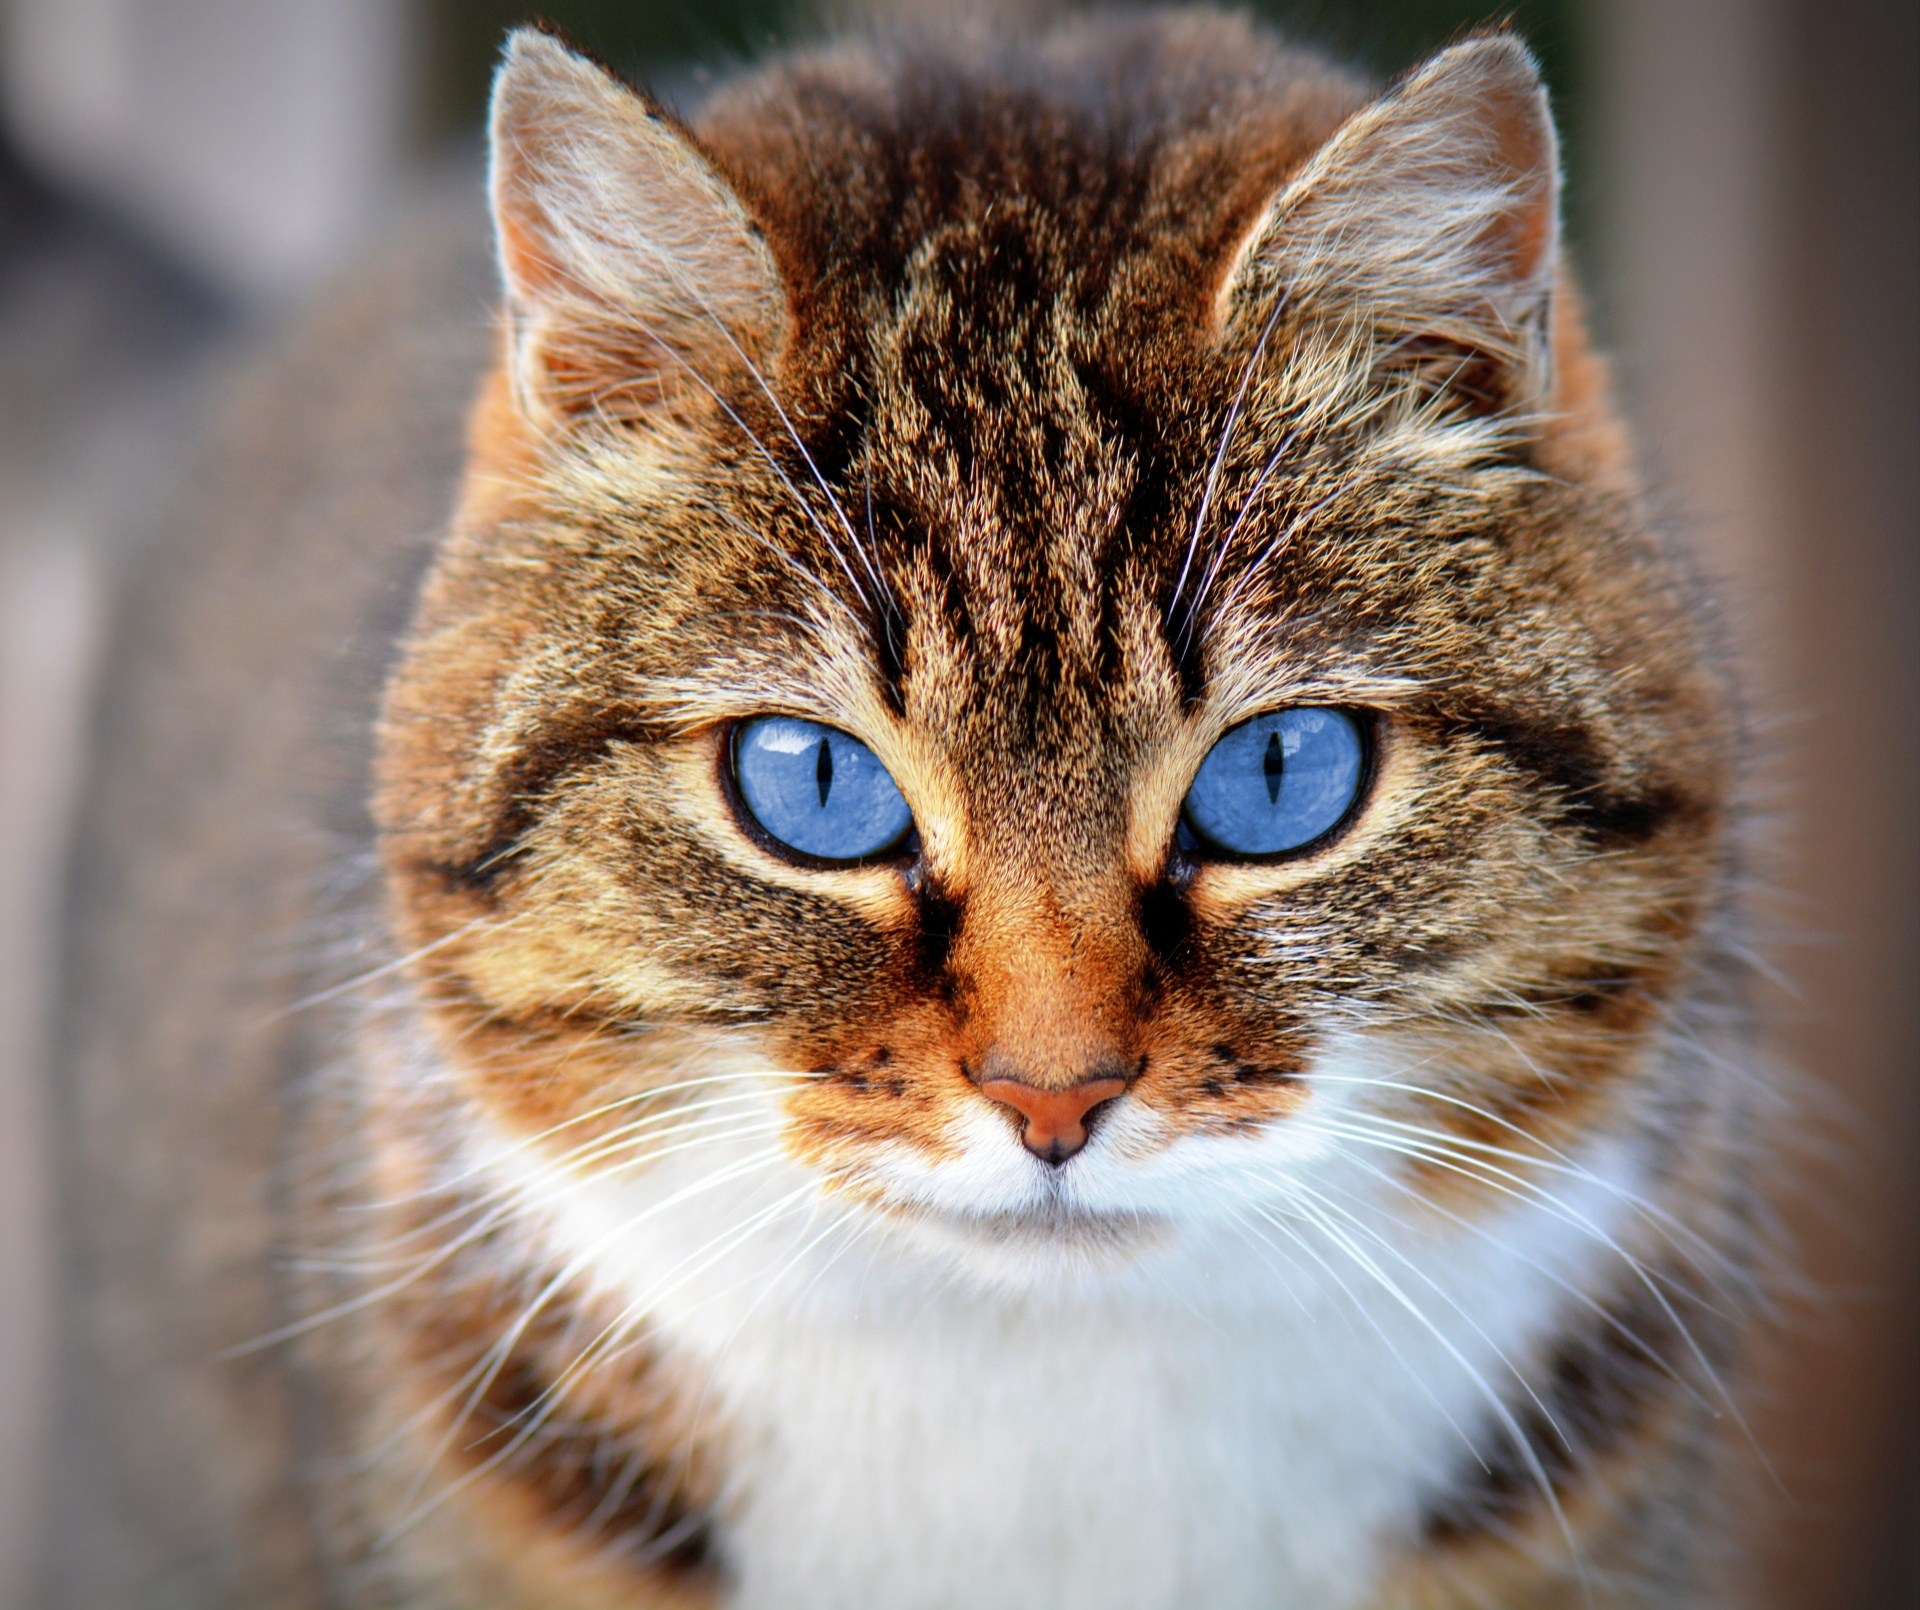
\includegraphics[height=27mm, trim=120mm 0mm 57.5mm 0mm, clip]{1_Example_Content/Images/cat-with-blue-eyes-15122819490rC.jpg}%
				%}%
			}%
		}%
	}%
	\hspace{15pt}%
	\textbf{\color{SpotColor}University of Bonn, Germany}
}
\bigskip


\begin{topic}

	%\item[\multiline{Mail {\normalsize\\} Phone · E-mail {\normalsize\\} WWW}]
	%\item
	\item[\multiline{%
		\icon{map} {\normalsize\\}% \icon{envelope} {\normalsize\\}
		\icon{comments} {\normalsize\\}%
		\icon{address-card}%
	}]
	Adenauerallee~24--42, 53113~Bonn, Germany \\
	+49~228~73-9288 · \email{holger.gerhardt@uni-bonn.de} \\
	\url{https://www.iame.uni-bonn.de/people/holger-gerhardt}

\end{topic}


\section{Professional experience}

\begin{topic}

	\item[\textbf{2011--present}]
	Postdoctoral Researcher, Center for Economics and Neuroscience and Institute for Applied Microeconomics, and Lab Manager, Bonn\-Econ\-Lab, University of Bonn, Germany.

	\item[2005--2011]
	Research and Teaching Assistant, Institute of Economic Policy, {\selectlanguage{ngerman}Humboldt-Universität zu Berlin,} Germany.

\end{topic}


\section{Academic education}

\begin{topic}

	\item[\textbf{2005--2011}]
	{\selectlanguage{ngerman}Humboldt-Universität zu Berlin,} School of Business and Economics and Berlin School of Mind and Brain, Dr.~rer.~pol. (Ph.D. in Economics), \textit{summa cum laude}. Dissertation: \textit{Essays in Experimental and Neuroeconomics}. Thesis advisors: Professor Lutz Weinke (economics) and Professor Hauke~R. Heekeren (neuroscience).

	\item[1999--2004]
	{\selectlanguage{ngerman}Humboldt-Universität zu Berlin,} School of Business and Economics, {\selectlanguage{ngerman}Diplom-Volkswirt} (Diploma in Economics, M.Sc.-equivalent). Diploma thesis: \textit{Reference-Dependent Consumer Preferences and Price Setting}. Awarded the \caps{WWG} Prize for the best diploma degree completed in the 2004/05 winter term.

\end{topic}


\section{Publications}

\begin{topic}

	%\begin{refcontext}[sorting=ydnt]
		% Sort BIBLIOGRAPHY by YEAR
	\begin{refcontext}[sorting=none]
		% Sort BIBLIOGRAPHY by APPEARANCE
	\nocite{Gerhardt2017}
	\nocite{Marsh2017}
	\nocite{Behrens2017}
	\nocite{Strang2017}
	\nocite{Schulreich2016}
	\nocite{Marsh2015}
	\nocite{Schulreich2014}

	\item[\textbf{Peer-reviewed articles}]
	\printbibliography[heading=none]
	\end{refcontext}
	
	\item[Book chapter]
	Antoine, Nadja M., and Holger Gerhardt. 2014. {\selectlanguage{ngerman}``Bestätigende und herausfordernde Impulse in der kokreativen Interaktion. Kokreative Wertschöpfung unter den Bedingungen von Koopetition am Beispiel der Ideenplattform jovoto,'' in: Klein, Inga and Sonja Windmüller (eds.), \textit{Kultur der Ökonomie. Zur Materialität und Performanz des Wirtschaft\-lichen, Edition Kulturwissenschaft}. transcript Verlag, Bielefeld,} Germany, \mbox{pp. 259--281}.
	\item[Doctoral dissertation]
	Gerhardt, Holger. 2013. \textit{Essays in Experimental and Neuro\-economics}. {\selectlanguage{ngerman}Humboldt-Universität zu Berlin,} School of Business and Economics. \url{https://edoc.hu-berlin.de/dissertationen/gerhardt-holger-2011-06-20}.

\end{topic}


\section{Current research projects}

\begin{topic}

	\item[\highlight{Job market paper}]
	Dertwinkel-Kalt, Markus, Holger Gerhardt, Gerhard Riener, \mbox{Frederik} Schwerter, and Louis Strang. ``Concentration Bias in \mbox{Intertemporal} Choice.'' \url{https://www.dropbox.com/s/dv20mcu0qkygmjz/ Concentration_Bias_in_Intertemporal_Choice.pdf}. Revise and resubmit, \textit{Review of Economic Studies}.

	\item[Work in progress]
	Gerhardt, Holger, and Rafael Suchy: ``Estimating Time Preferences from Strictly Convex Budgets.''
	
	Gerhardt, Holger, Guido Biele, Hauke R. Heekeren, and Harald \mbox{Uhlig}. ``Cognitive Load Increases Risk Aversion.'' SFB~649 \mbox{Discussion} Paper No.~2016-011. \url{https://sfb649.wiwi.hu-berlin.de/papers/pdf/ SFB649DP2016-011.pdfs}.
\end{topic}


\section{Teaching experience}

\begin{topic}

	\item[University of Bonn]
	Lecture ``Economics and Psychology'' (joint with Frederik Schwer\-ter), 2015/16, M.Sc. level.
	
	Lecture {\selectlanguage{ngerman}``Experimentelle Wirtschaftsforschung''} (in German, ``Ex\-peri\-mental Economics,'' joint with Sebastian Kube), 2014, B.Sc. level.
	
	Workshop ``Introduction to the software `PsychoPy','' 2019 (Master in Neuroscience program).

	Workshop ``Introduction to the software `Presentation','' 2011, 2014--2018 (Master in Neuroscience program).

	\item[\multiline{Humboldt-Universität \\ zu~Berlin}]

	Exercise classes to the lecture {\selectlanguage{ngerman}``Makroökonomie~I''} (in German, ``Macro\-economics~I''), B.Sc. level, 2008, 2009/10, 2011.
	
	Exercise class to the lecture ``Monetary Economics,'' B.Sc. level, 2009/10.
	
	Exercise classes to the lecture ``Growth and Inequality in an Inter\-national Perspective,'' M.Sc. level, 2008, 2009.
	
	Workshop on neuroeconomics: {\selectlanguage{ngerman}``Ökonomische Rationalität und das Gehirn''} (in German, ``Economic Rationality and the Brain'') as part of the 7\textsuperscript{th} symposium of the {\selectlanguage{ngerman}Humboldt-Forum Wirtschaft,} 2007.
	
	Exercise classes to the lecture {\selectlanguage{ngerman}``Konjunktur- und Wachs\-tums\-politik/\hspace{0pt}Angewandte Makroökonomie''} (in German, ``Business Cycle and Growth Policy/\hspace{0pt}Applied Macroeconomics''), B.Sc. level, 2006, 2006/07, 2007/08.
	
	Seminar ``Bounded Rationality and Macroeconomics,'' M.Sc. level, winter 2005/06.

\end{topic}
	
	
\section{Services to the profession and community}

\begin{topic}

	\item[Referee for]
	\textit{American Economic Review}; \textit{European Economic Review}; \textit{Frontiers in Decision Neuroscience}; \textit{Journal of Economic Psychology}; \textit{Journal of Institutional and Theoretical Economics}; \textit{Journal of Neurophysiology}; \textit{Journal of Neuroscience, Psychology, and Economics}; \textit{Quantitative Economics}.

	\item[TeX templates]
	Available at \url{https://github.com/HolgerGerhardt/TeXTemplates}.

\end{topic}


\section{Miscellaneous}

\begin{topic}

	\item[Language skills]
	German---native. \\
	English, Hebrew---fluent. \\
	French, Latin---basic knowledge.
	
	\item [Software skills]	Mathematica, \caps{MATLAB}, R, Stata---advanced knowledge; Python---basic knowledge. \\
	\caps{FSL} (tool for fMRI data analysis)---advanced knowledge. \\
	z-Tree---expert knowledge; oTree, Presentation---advanced knowledge. \\
	hroot, \caps{ORSEE}---expert knowledge.

\end{topic}


\section{References}

\begin{topic}

	\item[\textbf{Professor Armin Falk}]
	University of Bonn and briq Institute, Bonn, Germany \\
	+49~228~3894-701 (personal assistant) · \email{armin.falk@briq-institute.org}

	\item[\textbf{Professor Sebastian Kube}]
	University of Bonn, Germany \\
	+49~228~73-9240 (secretary) · \email{kube@uni-bonn.de}

\end{topic}


\end{document}